\documentclass{amsart}

\usepackage{enumerate, amsmath, amsfonts, amssymb, amsthm, thmtools, wasysym, graphics, graphicx, xcolor, url, hyperref, hypcap, a4wide, pdflscape, multido, xargs, colortbl, multicol, multirow, calc, shuffle, hvfloat}
\hypersetup{colorlinks=true, citecolor=darkblue, linkcolor=darkblue}
%\usepackage[all]{xy}
\usepackage{tikz}
\usetikzlibrary{trees, decorations, decorations.markings, shapes, arrows, matrix, calc, fit, intersections, patterns, angles, cd}
\usepackage{tikz-qtree}
\usepackage{comment}
\usepackage{etex}
\usepackage{ulem}\normalem % to strike through a word
\usepackage[noabbrev,capitalise]{cleveref}
\setlength{\abovecaptionskip}{10pt}
\setlength{\belowcaptionskip}{5pt}

%\reserveinserts{50}
\graphicspath{{figures/}}
\makeatletter
\def\input@path{{figures/}}
\makeatother

%%%%%%%%%%%%%%%%%%%%%%%%%%%%%%%%%%%%%%

\title[Ornamentation lattices and intreeval hypergraphic lattices]{Ornamentation lattices and \\ intreeval hypergraphic lattices}

\author{Vincent Pilaud}
\address[V.~Pilaud]{Universitat de Barcelona \& Centre de Recerca Matemàtica, Barcelona}
\email{vincent.pilaud@ub.edu}
\urladdr{https://www.ub.edu/comb/vincentpilaud/}

\thanks{
VP was partially supported by the Spanish project PID2022-137283NB-C21 of MCIN/AEI/10.13039/501100011033 / FEDER, UE, by the Spanish--German project COMPOTE (AEI PCI2024-155081-2 \& DFG 541393733), by the Severo Ochoa and María de Maeztu Program for Centers and Units of Excellence in R\&D (CEX2020-001084-M), by the Departament de Recerca i Universitats de la Generalitat de Catalunya (2021 SGR 00697), and by the French--Austrian project PAGCAP (ANR-21-CE48-0020 \& FWF I 5788).
}


%%%%%%%%%%%%%%%%%%%%%%%%%%%%%%%%%%%%%%

% theorems
\newtheorem{theorem}{Theorem}[section]
\newtheorem{theoremA}{Theorem}
\renewcommand{\thetheoremA}{\Alph{theoremA}}
\crefname{theoremA}{Theorem}{Theorems}
\newtheorem{corollary}[theorem]{Corollary}
\newtheorem{proposition}[theorem]{Proposition}
\newtheorem{lemma}[theorem]{Lemma}
\newtheorem{conjecture}[theorem]{Conjecture}
\crefname{conjecture}{Conjecture}{Conjectures}
\newtheorem{conjectureA}{Conjecture}
\renewcommand{\theconjectureA}{\Alph{conjectureA}}
\crefname{conjectureA}{Conjecture}{Conjectures}
\crefname{conjectureA}{Conjecture}{Conjectures}

\theoremstyle{definition}
\newtheorem{definition}[theorem]{Definition}
\newtheorem{example}[theorem]{Example}
\newtheorem{remark}[theorem]{Remark}
\newtheorem{question}[theorem]{Question}
\newtheorem{notation}[theorem]{Notation}
\newtheorem{openproblem}[theorem]{Open problem}
\crefname{notation}{Notation}{Notations}


% newcommands
% math special letters
\newcommand{\R}{\mathbb{R}} % reals
\newcommand{\N}{\mathbb{N}} % naturals
\newcommand{\Z}{\mathbb{Z}} % integers
\newcommand{\I}{\mathbb{I}} % set of integers
\newcommand{\C}{\mathbb{C}} % set of summands
\renewcommand{\b}[1]{\boldsymbol{#1}} % bold
\renewcommand{\c}[1]{\mathcal{#1}} % bold
\newcommand{\cal}[1]{\mathcal{#1}} % cal

% math commands
\newcommand{\set}[2]{\left\{ #1 \;\middle|\; #2 \right\}} % set notation
\newcommand{\bigset}[2]{\big\{ #1 \;|\; #2 \big\}} % big set notation
\newcommand{\biggset}[2]{\bigg\{ #1 \;\bigg|\; #2 \bigg\}} % big set notation
\newcommand{\multiset}[2]{\left\{\!\!\left\{ #1 \;\middle|\; #2 \right\}\!\!\right\}} % multiset notation
\newcommand{\bigmultiset}[2]{\big\{\!\!\big\{ #1 \;|\; #2 \big\}\!\!\big\}} % big multiset notation
\newcommand{\ssm}{\smallsetminus} % small set minus
\newcommand{\dotprod}[2]{\langle #1 | #2 \rangle} % dot product
\newcommand{\symdif}{\triangle} % symmetric difference
\newcommand{\one}{{1\!\!1}} % the all one vector
\newcommand{\eqdef}{\mbox{\,\raisebox{0.2ex}{\scriptsize\ensuremath{\mathrm:}}\ensuremath{=}\,}} % :=
\newcommand{\defeq}{\mbox{~\ensuremath{=}\raisebox{0.2ex}{\scriptsize\ensuremath{\mathrm:}} }} % =:
\newcommand{\polar}{^\diamond} % polar
\newcommand{\simplex}{\triangle} % simplex
%\renewcommand{\implies}{\;\Rightarrow\;} % implies

% operators
\DeclareMathOperator{\conv}{conv} % convex hull
\DeclareMathOperator{\cone}{cone} % cone hull
\DeclareMathOperator{\arr}{Arr} % arrangements
\DeclareMathOperator{\Inv}{Inv} % inversion set
\DeclareMathOperator{\Ninv}{Ninv} % non-inversion set
\DeclareMathOperator{\DemazureProduct}{Dem} % non-inversion set

% others
\newcommand{\fix}[1]{{\bf FIXME: }#1} % emphasis of a problem to FIX
\newcommand{\ie}{\textit{i.e.}~} % id est
\newcommand{\eg}{\textit{e.g.}~} % exempli gratia
\newcommand{\Eg}{\textit{E.g.}~} % exempli gratia
\newcommand{\aka}{\textit{aka.}~} % also known as
\newcommand{\viceversa}{\textit{vice versa}} % vice versa
\newcommand{\ordinal}{\textsuperscript{th}} % th for ordinals
\newcommand{\ex}[1]{^{\textrm{ex#1}}} % example
\newcommand{\para}[1]{\medskip\noindent\textbf{#1}} % paragraph
\newcommand{\subpara}[1]{\smallskip\noindent\textit{#1.}} % paragraph
\definecolor{darkblue}{rgb}{0,0,0.7} % darkblue color
\newcommand{\blue}[1]{{\color{blue} #1}} % blue
\newcommand{\red}[1]{{\color{red} #1}} % red
\newcommand{\darkblue}{\color{darkblue}} % darkblue command
\newcommand{\defn}[1]{\textsl{\darkblue #1}} % emphasis of a definition
\usepackage{todonotes}
\newcommand{\nantel}[1]{\todo[size=\tiny,color=red!30]{ #1 \\ \hfill --- N.}\,}
\newcommand{\Nantel}[1]{\todo[inline,color=red!30]{#1 \\ \hfill --- N.}}
\newcommand{\vincent}[1]{\todo[size=\tiny,color=blue!30]{ #1 \\ \hfill --- V.}\,}
\newcommand{\Vincent}[1]{\todo[inline,color=blue!30]{#1 \\ \hfill --- V.}}

% permutations
\newcommand{\fS}{\mathfrak{S}} % symmetric group
\newcommand{\fR}{\mathfrak{R}} % subset symmetric group


% lattices
\newcommand{\meet}{\wedge} % meet
\newcommand{\join}{\vee} % join
\newcommand{\bigMeet}{\bigwedge} % meet
\newcommand{\bigJoin}{\bigvee} % join
\newcommand{\less}{\vartriangleleft} % smaller WOIP
\newcommand{\lesseq}{\trianglelefteq} % smaller WOIP
\newcommand{\more}{\vartriangleright} % larger WOIP
\newcommand{\contactLess}[1]{\less_{#1}} % smaller contact graph
\newcommand{\contactMore}[1]{\more_{#1}} % larger contact graph
\newcommand{\projDown}{\pi^\downarrow} % Down projection
\newcommand{\projUp}{\pi^\uparrow} % Down projection

% Orientation, Hypergraph and Intervals
\newcommand{\Or}{\mathcal O}  % The map S_n --> acyclic orientation corresponding to vertices
\newcommand{\HH}{\mathbb H}  % general hypergraph
\newcommand{\II}{\mathbb I} % interval hypergraph
\newcommand{\cJ}{\cal{J}} % basic irreducibles index set
\newcommand{\cIJ}{\cal{IJ}} % basic irreducibles index set
\newcommand{\cX}{\cal{X}}
\newcommand{\cY}{\cal{Y}}
\newcommand{\cA}{\cal{A}}

% Special graphs
\newcommand{\Igraph}{\sf I} % I graph
\newcommand{\Ngraph}{\sf N} % N graph
\newcommand{\Xgraph}{\sf X} % X graph
\newcommand{\Ygraph}{\sf Y} % Y graph
\newcommand{\Dgraph}{\boldsymbol{\Diamond}} % D graph
\newcommand{\Agraph}{\rotatebox[origin=c]{180}{\sf Y}} % A graph

%%%%%%%%%%%%%%%%%%%%%%%%%%%%%%%%%%%%%%
%%%%%%%%%%%%%%%%%%%%%%%%%%%%%%%%%%%%%%
%%%%%%%%%%%%%%%%%%%%%%%%%%%%%%%%%%%%%%

\begin{document}

\begin{abstract}
\end{abstract}

\maketitle

\tableofcontents

%%%%%%%%%%%%%%%%%%%%%%%%%%%%%%%%%%%%%%
%%%%%%%%%%%%%%%%%%%%%%%%%%%%%%%%%%%%%%
%%%%%%%%%%%%%%%%%%%%%%%%%%%%%%%%%%%%%%

\pagebreak

\section{Introduction}
\label{sec:introduction}

\vincent{This is the introduction of the other paper. Needs to be updated...}
Fix an integer~$n \ge 1$ and denote by~$(\b{e}_i)_{i \in [n]}$ the standard basis of~$\R^n$.
The \defn{hypergraphic polytope} of a hypergraph~$\HH$ on~$[n]$ is the Minkowski sum
\(
\simplex_\HH \eqdef \sum_{H\in \HH} \simplex_H\,,
\)
where $\simplex_H$ is the simplex given by the convex hull of the points $\b{e}_h$ for~$h \in H$.
The face lattice of~$\simplex_\HH$ was described combinatorially in terms of acyclic orientations of~$\HH$ in~\cite{BenedettiBergeronMachacek}.
Note that the singletons of~$\HH$ are irrelevant for the combinatorics of~$\triangle_\HH$ as they just contribute to translations.
It is convenient for us to assume that~$\{i\} \in \HH$ for all~$i \in [n]$.

The \defn{hypergraphic poset}~$P_\HH$ is the transitive closure of the skeleton of~$\simplex_\HH$ oriented in the direction~$\b{\omega} \eqdef (n, n-1, \dots, 2, 1) - (1, 2, \dots, n-1, n) = (n-1, n-3, \dots, 3-n, 1-n)$.
For instance, 
\begin{itemize}
\item if~$\HH = \binom{[n]}{2}$ is the complete graph (or any hypergraph containing it), then~$\simplex_\HH$ is the \defn{permutahedron} and $P_\HH$ is the \defn{weak order on permutations},
\item if~$\HH = \set{[i,j]}{1 \le i \le j \le n}$ is the complete interval hypergraph, then~$\simplex_\HH$ is \mbox{J.-L.~Loday's} \defn{associahedron}~\cite{ShniderSternberg,Loday} and~$P_\HH$ is the \defn{Tamari lattice on binary trees}~\cite{Tamari}.
\end{itemize}

In view of these two examples, we would like to characterize the hypergraphs~$\HH$ for which $P_\HH$ is a lattice, a distributive lattice, a semidistributive lattice, a congruence-uniform lattice, a \mbox{(semi-)lattice} quotient of the weak order on permutations, etc.
These questions were settled in~\cite{Pilaud-acyclicReorientationLattices} for graphical zonotopes (\ie when~$\HH \subseteq \binom{[n]}{2}$), and also partially studied in~\cite{BarnardMcConville} for graph associahedra~\cite{CarrDevadoss} (\ie when~$\HH$ is the set of all subsets of vertices that induce a connected subgraph of a fixed graph on~$[n]$).

In this paper, we study the case of \defn{interval hypergraphs}~$\II$, \ie when all hyperedges of~$\II$ are intervals of~$[n]$.
Note that the family of interval hypergraphic polytopes does not contain the permutahedron, but contains
\begin{itemize}
\item the classical associahedron of~\cite{ShniderSternberg,Loday} when~$\II$ contains all intervals of~$[n]$,
\item the Pitman--Stanley polytope~\cite{PitmanStanley} when~$\II$ is the set of all singletons~$\{i\}$ and all initial intervals~$[i]$~for~${i \in [n]}$,
\item the freehedron of~\cite{Saneblidze-freehedron} when~$\II$ is the set of all singletons~$\{i\}$, all initial intervals~$[i]$ for~${i \in [n]}$, and all final intervals~$[n] \ssm [i]$~for~${i \in [n-1]}$,
\item the fertilitopes of~\cite{Defant-fertilitopes} when any two intervals of~$\II$ are either nested or disjoint.
\end{itemize}
In fact, it follows from~\cite{BazierMatteChapelierLaguetDouvilleMousavandThomasYildirim,PadrolPaluPilaudPlamondon} that the interval hypergraphic polytopes are precisely the weak Minkowski summands of the classical associahedron (recall that a polytope~$P \subset \R^n$ is a \defn{weak Minkowski summand} of a polytope~$Q \subset \R^n$ if there exists a real~$\lambda \ge 0$ and a polytope~$R \subset \R^d$ such that~$\lambda Q = P + R$).

We obtain the following characterizations, where we assume that~$\{i\} \in \II$ for all~$i \in [n]$ as mentioned earlier.
See \cref{sec:LatticeI,sec:distributive,sec:semidistributive,sec:quotient} and \cref{fig:notLattices,fig:Tamari,fig:distributiveLattices,fig:semidistributiveLattices,fig:notSemidistributiveLattices} for illustrations.

\begin{theoremA}
\label{thm:latticeI}
For an interval hypergraph $\II$, the poset $P_\II$ is a lattice if and only if $\II$ is closed under intersection (\ie $I, J \in \II$ and~$I \cap J \ne \varnothing$ implies~$I \cap J \in \II$).
\end{theoremA}

%\begin{theoremA}
%\label{thm:distributiveLatticeI}
%For an interval hypergraph $\II$, the poset $P_\II$ is a distributive lattice if and only if for all~$I, J \in \II$ such that~$I \not\subseteq J$, $I \not\supseteq J$ and~$I \cap J \ne \varnothing$, the intersection~$I \cap J$ is in~$\II$ and is initial or final in any~$K \in \II$ with~$I \cap J \subseteq K$.
%\end{theoremA}
%
%\begin{theoremA}
%\label{thm:semidistributiveLatticeI}
%For an interval hypergraph $\II$, the poset $P_\II$ is a join semidistributive lattice if and only if~$\II$ is closed under intersection and for all~$[r,r'], [s,s'], [t,t'], [u,u'] \in \II$ such that ${r < s \le r' < s'}$, $r < t \le s' < t'$, $u < \min(s, t)$ and~$s' < u'$, there is~$[v,v'] \in \II$ such that~$v < s$ and~${s' < v' < t'}$.
%A symmetric characterization holds for meet semidistributivity.
%\end{theoremA}
%
%\begin{theoremA}
%\label{thm:quotientLatticeI}
%For an interval hypergraph $\II$, the poset morphism from the weak order to the poset~$P_\II$ is a meet (resp.~join) semilattice morphism if and only if~$\II$ is closed under initial (resp.~final) subintervals (\ie~$[i,k] \in \II$ implies~$[i,j] \in \II$ (resp.~$[j,k] \in \II$) for any~$1 \le i < j < k \le n$).
%\end{theoremA}
%
%For instance, among the four above-mentioned families of interval hypergraphic polytopes, we recover that  the Pitman-Stanley polytope and all fertilitopes yield distributive lattices, the associahedron yields a semidistributive (but not distributive) lattice which is a quotient of the weak order, while the freehedron is not even a lattice (this was actually the motivation for~\cite{PilaudPoliakova} to construct alternative realizations of the skeleton of the freehedron).
%
%Once \cref{thm:latticeI} is established, an important step for \cref{thm:distributiveLatticeI,thm:semidistributiveLatticeI} is to understand join irreducible elements of~$P_\II$.
%\cref{subsec:joinIrreducibles} provides a combinatorial description of the join irreducible elements of the lattice~$P_\II$ for an arbitrary interval hypergraph~$\II$ closed under intersections.
%To prepare this slightly technical description, we already describe some join irreducible elements of~$P_\II$ in \cref{subsec:someJoinIrreducibles}, which happen to be all join irreducible elements of~$P_\II$ under the condition of~\cref{thm:distributiveLatticeI}.
%
%The paper is organized as follows.
%In \cref{sec:HP}, we recall basic properties of hypergraphic polytopes, we define hypergraphic posets, and we recall the natural poset morphism from the weak order on permutations to the hypergraphic poset~$P_\II$.
%In \cref{sec:IHP}, we develop specific properties of interval hypergraphic polytopes, in particular a simple characterization of their vertices and a global description of the relations in their hypergraphic posets.
%In \cref{sec:LatticeI}, we characterize the interval hypergraphs~$\II$ for which the interval hypergraphic poset~$P_\II$ is a lattice, proving \cref{thm:latticeI}.
%In \cref{sec:distributive}, we describe a family of join irreducible elements of~$P_\II$ and we characterize the interval hypergraphs~$\II$ for which~$P_\II$ is a distributive lattice, proving \cref{thm:distributiveLatticeI}.
%In \cref{sec:semidistributive}, we describe all join irreducible elements of~$P_\II$ and we characterize the interval hypergraphs~$\II$ for which~$P_\II$ is a join (or meet) semidistributive lattice, proving \cref{thm:semidistributiveLatticeI}.
%In \cref{sec:quotient}, we characterize the interval hypergraphs~$\II$ for which the poset morphism from the weak order on permutations to~$P_\II$ is a join (or meet) semilattice morphism, proving \cref{thm:quotientLatticeI}.

%%%%%%%%%%%%%%%%%%%%%%%%%%%%%%%%%%%%%%
%%%%%%%%%%%%%%%%%%%%%%%%%%%%%%%%%%%%%%
%%%%%%%%%%%%%%%%%%%%%%%%%%%%%%%%%%%%%%

\newpage
\section{Ornamentation lattices}

\begin{figure}
	\centerline{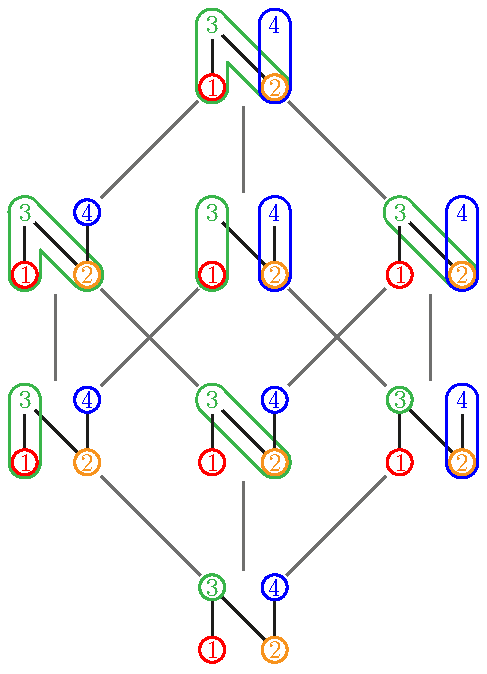
\includegraphics[scale=.8]{ornamentationsN} \qquad \raisebox{.5cm}{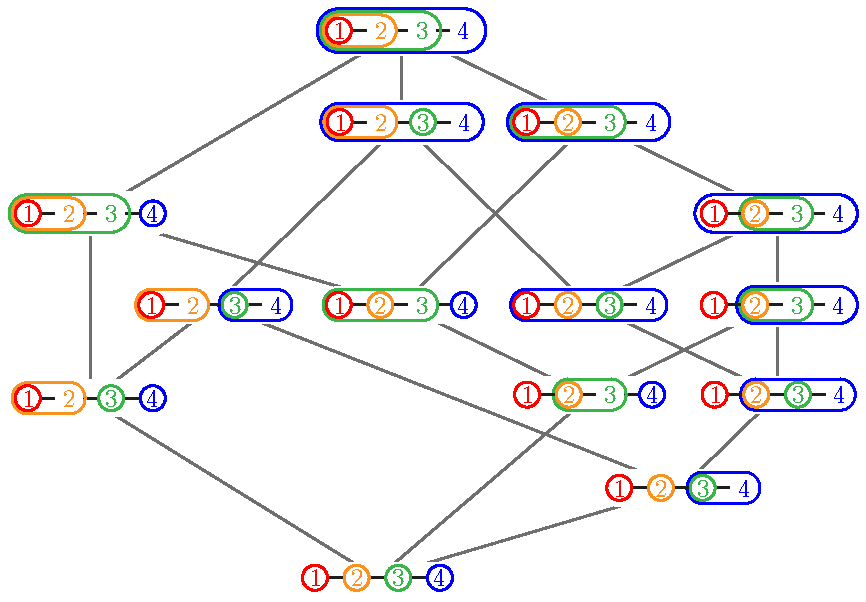
\includegraphics[scale=.8]{ornamentationsI}}}
	\caption{The ornamentation lattices~$\c{O}(\Ngraph)$ and~$\c{O}(\Igraph)$.}
	\label{fig:ornamentationsNI}
\end{figure}

\begin{figure}
	\centerline{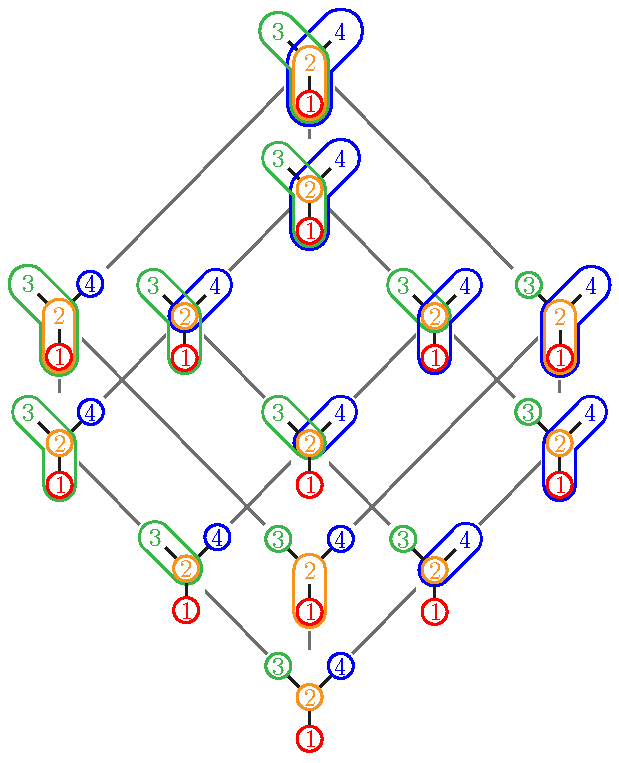
\includegraphics[scale=.8]{ornamentationsY} \qquad 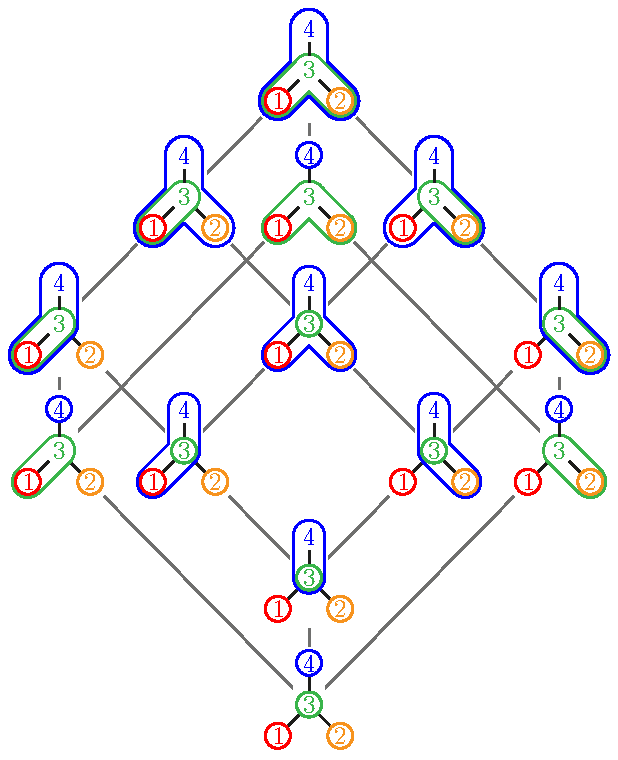
\includegraphics[scale=.8]{ornamentationsA}}
	\caption{The ornamentation lattices~$\c{O}(\Ygraph)$ and~$\c{O}(\Agraph)$.}
	\label{fig:ornamentationsAY}
\end{figure}

Throughout this section, we fix a directed graph~$D$ on a vertex set~$V$.
In all our pictures, $V = [n]$ and the edges are increasing (so we do not need to explicitly indicate the orientation).
%We will mostly work with a directed acyclic graph, and we represent it with edges going up in all pictures.
The following definition, first introduced for rooted trees in~\cite{} and extended to arbitrary directed graphs in~\cite{}, is illustrated in \cref{fig:ornamentationsNI,fig:ornamentationsAY,fig:ornamentationsX,fig:ornamentationsD}

\begin{definition}
An \defn{ornament} at a vertex $v$ of~$D$ is a subset~$U \subseteq V$ such that there is a path from any $u \in U$ to~$v$ in the directed subgraph of~$D$ induced by~$U$.
An \defn{ornamentation} of~$D$ is a map $O$ on $V$ which assigns an ornament~$O(v)$ at each vertex~$v \in V$ such that~$u \in O(v) \implies O(u) \subseteq O(v)$ for all~$u,v \in V$.
We denote by~$\c{O}(v \in D)$ the set of ornaments at a vertex~$v$ of~$D$ and by~$\c{O}(D)$ the set of ornamentations of~$D$.
\end{definition}

\begin{example}
We can define ornamentations by
\begin{itemize}
\item sending each vertex~$v \in V$ to the singleton~$\{v\}$, 
\item sending each vertex~$v \in V$ to the set~$U$ of vertices with a path to~$v$ in~$D$,
\item for any ornament~$U \in \c{O}(v \in D)$, sending~$v$ to~$U$ and any other vertex~$u \in V \ssm \{v\}$ to the singleton~$\{u\}$.
\end{itemize}
\end{example}

\begin{lemma}
\label{lem:unionOrnaments}
\begin{enumerate}[(i)]
\item If~$U \in \c{O}(u \in D)$ and~$U' \in \c{O}(u' \in D)$ with~$u \in U'$, then~${U \cup U' \in \c{O}(u' \in D)}$.
%\item If~$U$ is an ornament at a vertex~$u$ of~$D$ and~$U'$ is an ornament at a vertex~$u'$ of~$D$ and~$u \in U'$, then~$U \cup U'$ is an ornament of~$D$ at~$u'$.
\item If~$U,U' \in \c{O}(v \in D)$, then~$U \cup U' \in \c{O}(v \in D)$, while $U \cap U'$ is not necessarily in~$\c{O}(v \in D)$.
%\item If~$U,U'$ are two ornaments at a vertex~$v$ of~$D$, then~$U \cup U'$ is also an ornament at~$v$, while $U \cap U'$ is not necessarily an ornament at~$v$.
\end{enumerate}
\end{lemma}

\begin{proof}
For Part~(i), let~$w \in U \cup U'$. If~$w \in U'$, then there is a path from~$w$ to~$u'$ in~$U'$, hence in~$U \cup U'$.
If~$w \in U$, then there is a path from~$w$ to~$u$ in~$U$ and a path from~$u$ to~$u'$ in~$U'$, hence a path from~$w$ to~$u'$ in~$U \cup U'$.
Part~(ii) is a specialization of Part~(i) to~$u = v$ and~$u' = v$.
\end{proof}

\begin{theorem}
The set~$\c{O}(D)$ of ornamentations of~$D$ is a lattice under componentwise inclusion, meaning~$O_1 \le O_2$ if~$O_1(v) \subseteq O_2(v)$ for all~$v \in V$.
For any two ornamentations~$O_1$ and~$O_2$ of~$D$,
\begin{itemize}
\item $(O_1 \meet O_2)(v)$ is the inclusion maximal ornament at~$v$ contained in~$O_1(v) \cap O_2(v)$,
%\item the join~$O_1 \join O_2$ is the ornamentation of~$D$ where~$(O_1 \join O_2)(v) = \set{u \in V}{u \, R \, v}$ where $R$ is the transitive closure of~$u \in O_1(v) \cup O_2(v)$.
\item $(O_1 \join O_2)(v)$ is the inclusion minimal subset~$U$ of~$V$ containing~$v$ and such that~$u \in U$ implies~$O_1(u) \cup O_2(u) \subseteq U$.
\end{itemize}
\end{theorem}

\begin{proof}
%Given two ornamentations~$O_1$ and~$O_2$ of~$D$, let~$O_\meet$ and $O_\join$ be the maps on~$V$ defined by 
%\begin{itemize}
%\item $O_\meet(v)$ is the inclusion maximal ornament at~$v$ contained in~$O_1(v) \cap O_2(v)$,
%%\item $O_\join(v) = \set{u \in V}{u \, R \, v}$ where $R$ is the transitive closure of~$u \in O_1(v) \cup O_2(v)$.
%\item $O_\join(v)$ is the inclusion minimal subset~$U$ of~$V$ containing~$v$ and such that~$u \in U$ implies~$O_1(u) \cup O_2(u) \subseteq U$.
%\end{itemize}
%
Given two ornamentations~$O_1$ and~$O_2$ of~$D$, consider the map~$O_\meet$ on~$V$ where $O_\meet(v)$ is the inclusion maximal ornament at~$v$ contained in~$O_1(v) \cap O_2(v)$.
Note that $O_\meet(v)$ is well defined by \cref{lem:unionOrnaments}, and that~$O_\meet(v) \in \c{O}(v \in D)$ for any~$v \in V$ by definition.
Consider now~$u,v \in V$ such that~$u \in O_\meet(v)$.
Since~$O_\meet(u) \in \c{O}(u \in D)$ and~$O_\meet(v) \in \c{O}(v \in D)$ with~${u \in O_\meet(v)}$, \cref{lem:unionOrnaments} gives~$O_\meet(u) \cup O_\meet(v) \in \c{O}(v \in D)$.
As~$u \in O_\meet(v) \subseteq O_1(v) \cap O_2(v)$ and~$O_1$ and~$O_2$ are ornamentations of~$D$, we have~$O_1(u) \subseteq O_1(v)$ and~$O_2(u) \subseteq O_2(v)$, so that~$O_\meet(u) \subseteq O_1(u) \cap O_2(u) \subseteq O_1(v) \cap O_2(v)$, hence~$O_\meet(u) \cup O_\meet(v) \subseteq O_1(v) \cap O_2(v)$.
By maximality of~$O_\meet(v)$, we conclude that $O_\meet(u) \cup O_\meet(v) \subseteq O_\meet(v)$, so that~$O_\meet(u) \subseteq O_\meet(v)$.
We conclude that~$O_\meet$ is an ornamentation of~$D$.
Moreover, $O_\meet$ is clearly the meet of~$O_1$ and~$O_2$ in componentwise inclusion.

Given two ornamentations~$O_1$ and~$O_2$ of~$D$, consider now the map~$O_\join$ on~$V$ where~$O_\join(v)$ is the inclusion minimal subset~$U$ of~$V$ containing~$v$ and such that~$u \in U$ implies~$O_1(u) \cup O_2(u) \subseteq U$.
Note that~$O_\join(v)$ is well defined as it can be constructed by induction, starting from~$U = \{v\}$ and adding inductively~$O_1(u) \cup O_2(u)$ for all~$u \in U$ until it stabilizes.
Since~$O_1(u) \cup O_2(u) \in \c{O}(u \in D)$ by \cref{lem:unionOrnaments}, this inductive construction maintains the invariant that there is a path from~$u$ to~$v$ in~$U$ for any~$u \in U$.
Hence, we obtain that~$O_\join(v) \in \c{O}(v \in D)$ for any~$v \in V$.
Consider now~$u,v \in V$ such that~$u \in O_\join(v)$.
Since~$u \in O_\join(v)$ and~$w \in O_\join(v)$ implies~$O_1(w) \cup O_2(w) \subseteq O_\join(v)$, we obtain that~$O_\join(u) \subseteq O_\join(v)$ by minimality of~$O_\join(u)$.
We conclude that~$O_\join$ is an ornamentation of~$D$.
Moreover, $O_\join$ is clearly the join of~$O_1$ and~$O_2$ in componentwise inclusion.
\end{proof}

\begin{example}
The ornamentation lattice of the graph with a single edge is an $2$-elements chain.
The ornamentation lattice of a graph with no path of length $2$ is a boolean lattice (see \eg \cref{fig:ornamentationsNI}\,(left)).
In general, the Cartesian product~$\c{O}(D) \times \c{O}(D')$ of the ornamentation lattices of two directed graphs~$D$ and~$D'$~is
\begin{itemize}
\item the ornamentation lattice~$\c{O}(D \sqcup D')$ of the disjoint union of~$D$ and~$D'$, and
\item isomorphic to the ornamentation lattice~$\c{O}(D \sqcup D' / u \sim u')$ of the graph obtained from~${D \sqcup D'}$ by identifying a source (resp.~sink)~$u \in D$ with a source (resp.~sink)~$u' \in D'$.
\end{itemize}
\end{example}

\begin{example}
The ornamentation lattice of a $n$-elements path is isomorphic to the Tamari lattice on binary trees with $n$ nodes (see \eg \cref{fig:ornamentationsNI}\,(right)).
The isomorphism is obtained trough tubings (or equivalently bracket vectors).
\end{example}

\begin{remark}
\label{rem:posetPropertiesOrnamentations}
A few poset properties of the ornamentations lattice~$\c{O}(D)$:
\begin{itemize}
\item The minimal ornamentation sends each vertex~$v \in V$ to the singleton~$\{v\}$, and the maximal ornamentation sends each vertex~$v \in V$ to the set~$U$ of vertices with a path to~$v$ in~$D$.
\item Two ornamentations~$O_1$ and~$O_2$ of~$D$ form a cover relation if and only if there is~$u, v \in V$ such that~$u \notin O_1(v)$ and~$O_2(v) = O_1(u) \cup O_1(v)$, while~$O_1(w) = O_2(w)$ for all~$w \in V \ssm \{v\}$.
\item For any~$U \subseteq V$, the ornamentation lattice of the subgraph~$D_U$ of~$D$ induced by~$U$ is an interval of the ornamentation lattice of~$D$ (namely, the bottom interval below the ornamentation of~$D$ where~$O(u)$ is the set of vertices of~$U$ with a path to~$u$ in~$U$ for all~$u \in U$, while~$O(v)$ is the singleton~$\{v\}$ for all~$v \in V \ssm U$).
\end{itemize}
\end{remark}

\begin{remark}
A few lattice properties of the ornamentation lattice~$\c{O}(D)$:
\begin{itemize}
\item The join irreducible ornamentations of~$D$ are precisely the ornamentations~$\c{O}_\pi$ described in \cref{rem:posetPropertiesOrnamentations} for the directed paths~$\pi$ in~$D$ which admit no shortcut in~$D$. (The meet irreducible ornamentations are more complicated to describe.)
\item $\c{O}(D)$ is distributive if and only if~$D$ contains no path of length~$2$ (in which case, $\c{O}(D)$ is actually a boolean lattice).
\item $\c{O}(D)$ is semidistributive if and only if~$D$ is a directed tree.
\end{itemize}
\end{remark}

\begin{figure}[p]
	\centerline{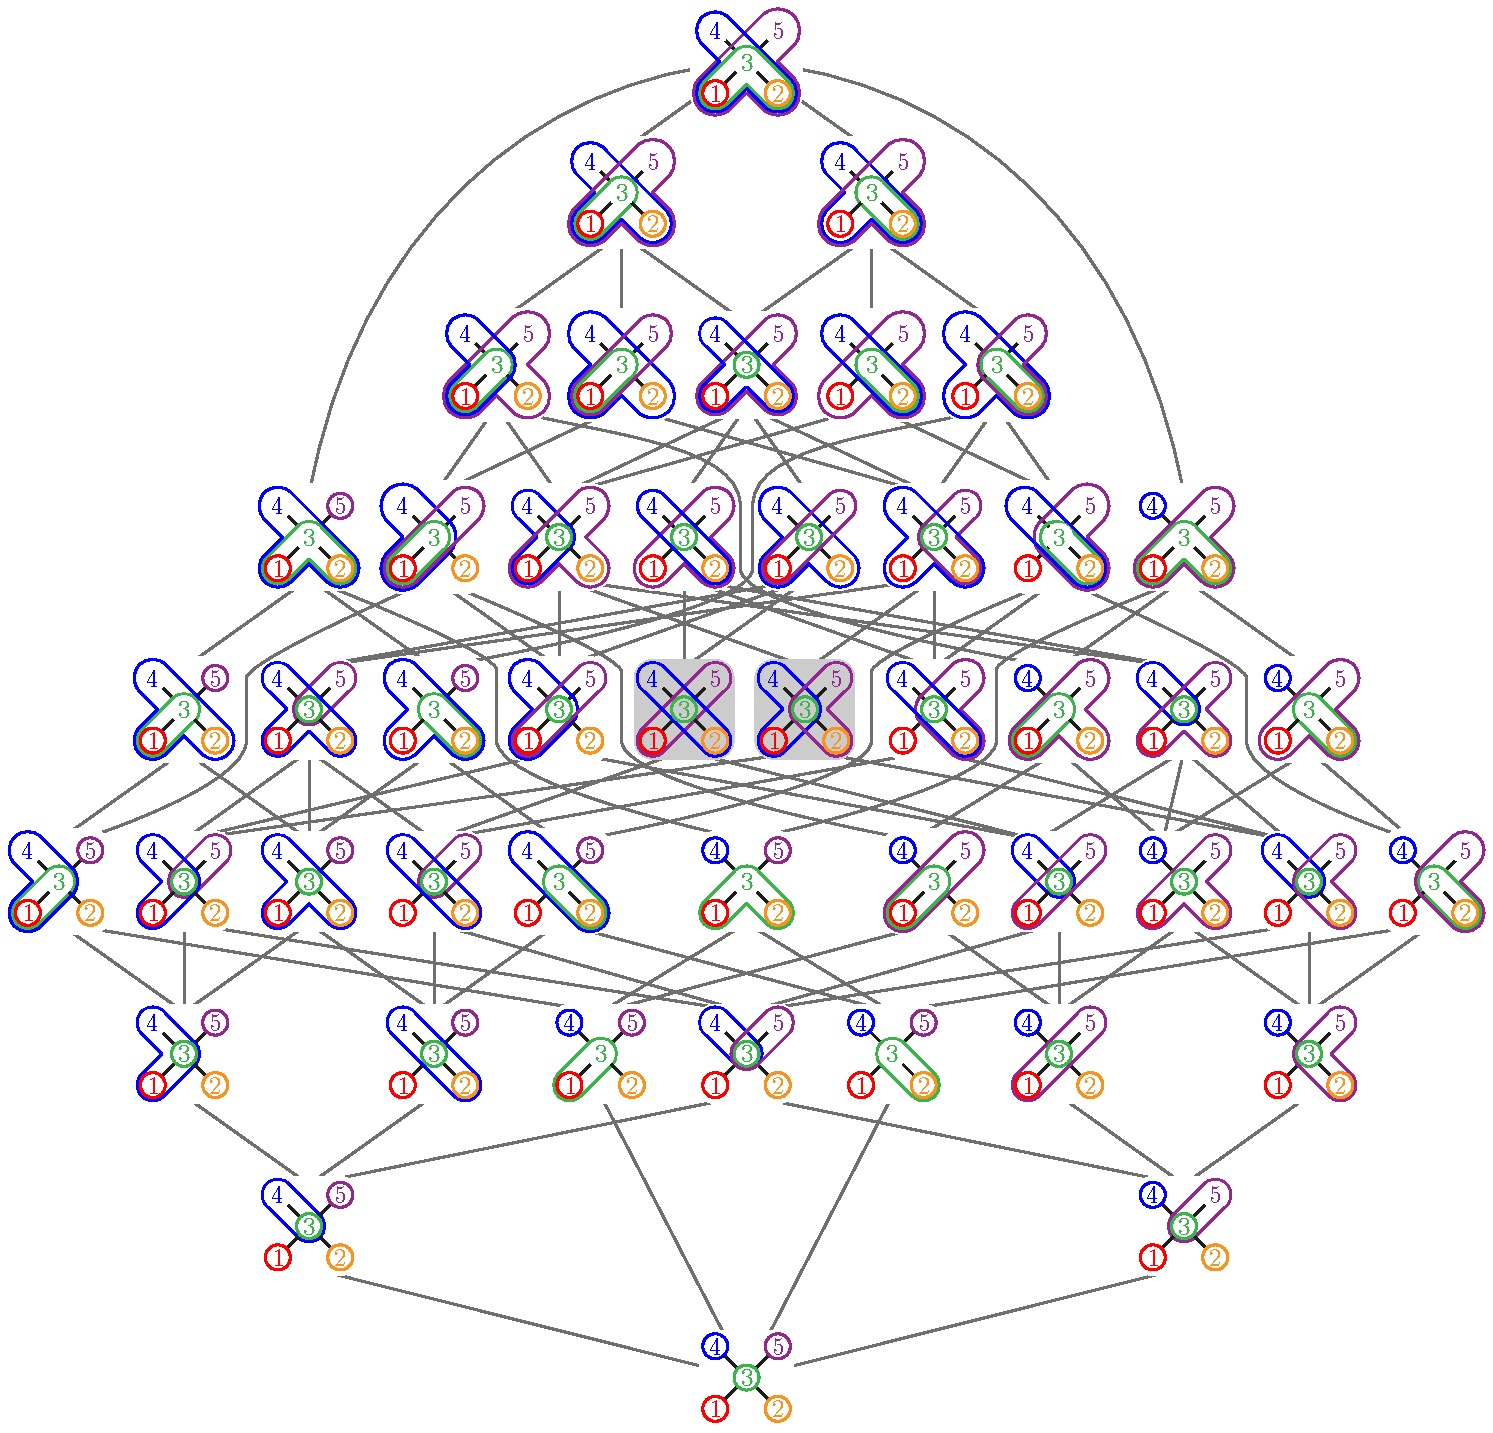
\includegraphics[scale=.8]{ornamentationsX}}
	\caption{The ornamentation lattice~$\c{O}(\Xgraph)$ of the directed graph~$\Xgraph$.}
	\label{fig:ornamentationsX}
\end{figure}

\begin{figure}
	\centerline{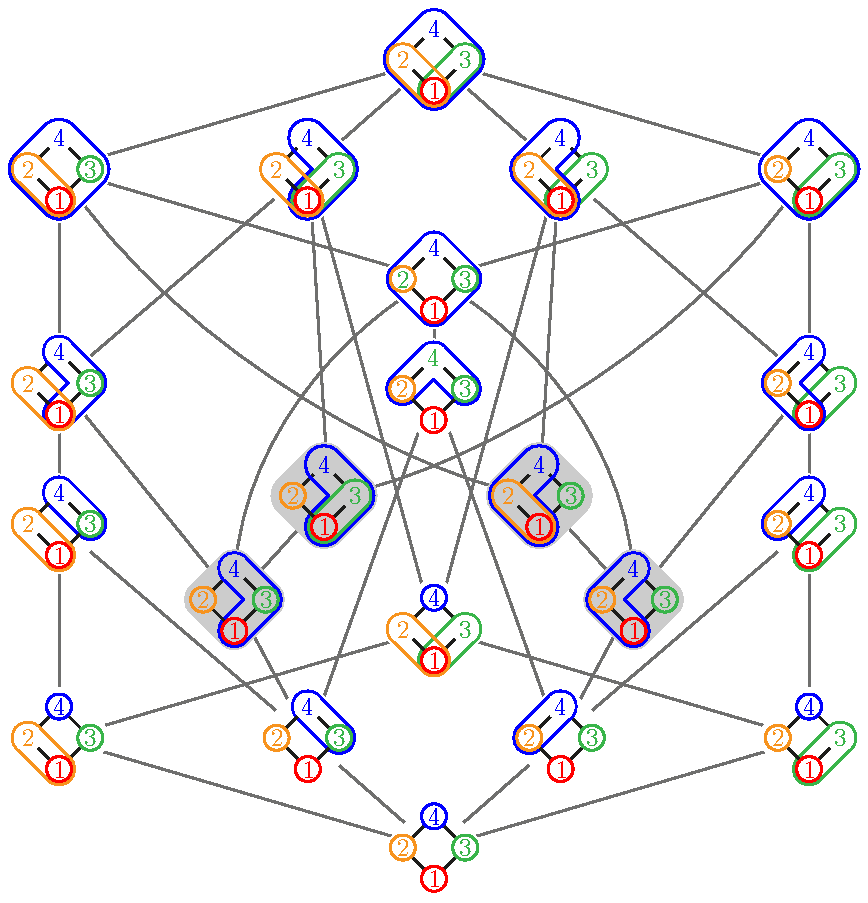
\includegraphics[scale=.8]{ornamentationsD}}
	\caption{The ornamentation lattice~$\c{O}(\Dgraph)$ of the directed graph~$\Dgraph$.}
	\label{fig:ornamentationsD}
\end{figure}

%%%%%%%%%%%%%%%%%%%%%%%%%%%%%%%%%%%%%%
%%%%%%%%%%%%%%%%%%%%%%%%%%%%%%%%%%%%%%
%%%%%%%%%%%%%%%%%%%%%%%%%%%%%%%%%%%%%%

\section{Intreeval lattices}

%%%%%%%%%%%%%%%%%%%%%%%%%%%%%%%%%%%%%%
%%%%%%%%%%%%%%%%%%%%%%%%%%%%%%%%%%%%%%
%%%%%%%%%%%%%%%%%%%%%%%%%%%%%%%%%%%%%%

\section{}

\end{document}

\setcounter{theoremA}{0}

%%%%%%%%%%%%%%%%%%%%%%%%%%%%%%%%%%%%%%
%%%%%%%%%%%%%%%%%%%%%%%%%%%%%%%%%%%%%%
%%%%%%%%%%%%%%%%%%%%%%%%%%%%%%%%%%%%%%

\section{Hypergraphic posets}
\label{sec:HP}

%%%%%%%%%%%%%%%%%%%%%%%%%%%%%%%%%%%%%%

\subsection{Hypergraphic polytopes}
\label{subsec:D_H}

A \defn{hypergraph} $\HH$ on $[n] \eqdef \{1, \dots, n\}$ is a collection of  subsets of~$[n]$.
By convention, we always assume that~$\HH$ contains all singletons~$\{i\}$ for~$i\in [n]$.
The \defn{hypergraphic polytope}~$\simplex_\HH$ is the Minkowski sum
\[
\simplex_\HH \eqdef \sum_{H\in \HH} \simplex_H\,,
\]
where $\simplex_H$ is the simplex given by the convex hull of the points $\b{e}_h \in \R^n$ for~$h \in H$.

\begin{example}
\label{exm:DH1}
For the hypergraph $\HH=\{ 1, 2, 3, 4, 123, 134 \}$,
we  have
\[
\begin{array}{ccc}
 \begin{tikzpicture}[scale=1,baseline=.5cm]
	\node (1) at (0.6,1.0) {$\scriptstyle e_1$};
	\node (2) at (-.2,-.2) {$\scriptstyle e_2$};
	\node (3) at (1.3,-.2) {$\scriptstyle e_3$};
	\draw [fill=blue!40] (0,0) -- (.6,.75) -- (1.2,0) --(0,0) ;   % e2--e1--e3--e2
\end{tikzpicture} \quad &
 \begin{tikzpicture}[scale=1,baseline=.5cm]
	\node (1) at (0.6,1.0) {$\scriptstyle e_1$};
	\node at (1.3,-.2) {$\scriptstyle e_3$};
	\node at (2.4,.5) {$\scriptstyle e_4$};
	\draw [fill=green!20] (1.2,0) -- (2.2,.5 )--(.6,.75)--(1.2,0); %  e3--e4--e1--e3
\end{tikzpicture} \quad &
\begin{tikzpicture}[scale=1,baseline=.5cm]
	\draw [color=gray!10,fill=blue!2] (1.6,1.25)--(1,.5)--(2.2,.5)-- (1.6,1.25); 
	\draw [color=gray!10,fill=green!5]  (0,0)--(1,.5)--(-.6,.75)--(0,0);
	\draw [dotted,color=green] (0,0)--(1,.5)--(-.6,.75);
	\draw [dotted,color=blue] (1.6,1.25)--(1,.5)--(2.2,.5);
	\draw (0,1.5)-- (1.6,1.25) -- (2.2,.5) -- (1.2,0) --(0,1.5) ; 
	\draw (0,0)--(-.6,.75)--(0,1.5)-- (1.2,0) --(0,0); 
\end{tikzpicture}\\
\blue{\simplex_{123}}& \green{\simplex_{134}} & \simplex_\HH = \simplex_1 + \simplex_2 + \simplex_3 + \simplex_4 + \blue{\simplex_{123}} + \green{\simplex_{134}}\\
\end{array}
\]
which is a 3-dimensional polytope sitting in $\R^4$.
Note that as~$n \le 9$ in all our examples, we simplify notations and write~$123$ for the set~$\{1,2,3\}$.
\end{example}

\begin{remark}
\label{rem:single}
Note that the singletons hyperedges are irrelevant for our purposes.
Namely, adding to~$\HH$ the hyperedge~$\{i\}$ for some~$i \in [n]$ just translates the polytope~$\simplex_\HH$ in the direction~$\b{e}_i$, which does not affect the face structure of the polytope.
For our conditions on hypergraphs of \cref{thm:latticeI,thm:distributiveLatticeI}, it is convenient for us to assume that $\{i\} \in \HH$ for all $i \in [n]$.
When quoting results from~\cite{BenedettiBergeronMachacek}, the reader will have to be mindful that they took the opposite convention.
\end{remark}


%%%%%%%%%%%%%%%%%%%%%%%%%%%%%%%%%%%%%%

\subsection{Acyclic orientations, increasing flips, and hypergraphic posets} 
\label{subsec:P_H}

We now recall from \cite[Thm.~2.18]{BenedettiBergeronMachacek} a combinatorial model for the graph~$(V_\HH, E_\HH)$ of~$\simplex_\HH$.
As we are only interested in the $1$-skeleton of~$\simplex_\HH$, we simplify some of the general definitions of~\cite{BenedettiBergeronMachacek} which were designed to deal with all faces of~$\simplex_\HH$.

\begin{definition}
\label{def:acyclicOrientation}
An \defn{orientation} of~$\HH$ is a map~$O$ from~$\HH$ to~$[n]$ such that~$O(H) \in H$ for all~${H \in \HH}$.
Equivalently, we often represent the orientation~$O$ as the set of pairs~$\set{(O(H),H)}{H \in \HH}$.
The orientation~$O$ is \defn{acyclic} if there is no~$H_1, \dots, H_k$ with~$k \ge 2$ such that~$O(H_{i+1}) \in H_i \ssm \{O(H_i)\}$ for~$i \in [k-1]$ and~$O(H_1) \in H_k \ssm \{O(H_k)\}$.
\end{definition}

\begin{remark}
The singleton~$\{i\}$ of~$\HH$ is always oriented $O(\{i\})=i$, and plays no role in determining  the acyclicity of~$O$ since $\{i\} \ssm \{O(\{i\})\} = \varnothing$.
We will therefore omit the singletons when describing or drawing orientations (see also~\cref{exm:intervalHypergraph}).
If we list the non-singleton elements $(H_1,H_2,...,H_k)$ of $\HH$ in some fixed order, it is then convenient to describe an orientation~$O$ as the tuple $O=(O(H_1),O(H_2),\ldots,O(H_k))$. 
\end{remark}

\begin{example}
\label{exm:DH2}
Using $\HH=\{ 1, 2, 3, 4, 123, 134 \}$ as in~\cref{exm:DH1}, we order the two non-singleton $(123,134)$.
There are $9$ orientations of~$\HH$, $7$ of which are acyclic as displayed in~\cref{fig:Orientation1}. 
For instance, the orientation $(O(123), O(134)) = (1,3)$ is cyclic since $O(123) = 1 \in 134$ and $O(134) = 3 \in 123$ is a cycle with $k = 2$.
%
\begin{figure}
	\centerline{
	\begin{tabular}{c@{\qquad}c}
		\begin{tikzpicture}[scale=2,baseline=.5cm]
		\draw [color=gray!10,fill=blue!2] (1.6,1.25)--(1,.5)--(2.2,.5)-- (1.6,1.25); 
		\draw [color=gray!10,fill=green!5]  (0,0)--(1,.5)--(-.6,.75)--(0,0);
		\node (23) at (0,0) {$\scriptstyle (2,3)$}; 		
		\node (21) at (-.6,.75) {$\scriptstyle (2,1)$};	
		\node (24) at (1,.5) {$\scriptstyle (2,4)$}; 	
		\node (34) at (2.2,.5) {$\scriptstyle (3,4)$};
		\node (14) at (1.6,1.25) {$\scriptstyle (1,4)$};	
		\node (33) at (1.2,0) {$\scriptstyle (3,3)$};	
		\node (11) at (0,1.5) {$\scriptstyle (1,1)$};		
		\path[color=red, ->] (11) edge node[fill=white,inner sep=2pt, font=\tiny ] {$  12 $} (21);
		\path[color=red, ->] (11) edge node[fill=white,inner sep=2pt, font=\tiny ] {$  13 $} (33);
		\path[color=red, ->] (11) edge node[fill=white,inner sep=2pt, font=\tiny ] {$  14 $} (14);
		\path[color=red, ->] (14) edge node[fill=white,inner sep=2pt, font=\tiny ] {$  13 $} (34) ;
		\path[dotted,color=red, ->] (14) edge node[fill=white,inner sep=2pt, font=\tiny ] {$  12 $} (24)  ;
		\path[dotted,color=red, ->] (24) edge node[fill=white,inner sep=2pt, font=\tiny ] {$  23 $} (34)  ;
		\path[dotted,color=red, ->] (21) edge node[fill=white,inner sep=2pt, font=\tiny ] {$  14$} (24);
		\path[color=red, ->] (21) edge node[fill=white,inner sep=2pt, font=\tiny ] {$  13$} (23);
		\path[dotted,color=red, <-]  (24) edge node[fill=white,inner sep=2pt, font=\tiny ] {$  34$} (23);
		\path[color=red, ->]  (23) edge node[fill=white,inner sep=2pt, font=\tiny ] {$  23$} (33);
		\path[color=red, ->]  (33) edge node[fill=white,inner sep=2pt, font=\tiny ] {$  34$} (34);
		\end{tikzpicture}
	&
		\begin{tikzpicture}[scale=1,baseline=.5cm]
		\node (11) at (0,0) {$\scriptstyle (1,1)$};
		\node (21) at (-1,1) {$\scriptstyle (2,1)$};	
		\node (23) at (-1,2) {$\scriptstyle (2,3)$}; 		
		\node (14) at (1,1.5) {$\scriptstyle (1,4)$};	
		\node (24) at (0,3) {$\scriptstyle (2,4)$}; 	
		\node (33) at (-2,3) {$\scriptstyle (3,3)$};
		\node (34) at (-1,4) {$\scriptstyle (3,4)$};	
		\draw (11)--(21);
		\draw (11)--(14);
		\draw (21)--(23);
		\draw (23)--(24);
		\draw (14)--(24);
		\draw (23)--(33);
		\draw (33)--(34);
		\draw (24)--(34);
		\end{tikzpicture}
	\\
	$\Delta_\HH$ & $P_\HH$\\
	\end{tabular}
	}
	\caption{The polytope $\Delta_{\HH}$ for $\HH=\{ 1, 2, 3, 4, 123, 134 \}$ has seven vertices corresponding to the acyclic orientations of $\HH$ and eleven (oriented) edges corresponding to the increasing flips between these orientations.
	The poset $P_\HH$ is the transitive closure of the increasing flip graph.}
	\label{fig:Orientation1}
\end{figure}
\end{example}

\begin{definition}
\label{def:flip}
Two orientations~$O \ne O'$ of~$\HH$ are related by an \defn{increasing flip} if there exist~${1 \le i < j \le n}$ such that for all~$H \in \HH$, 
\begin{itemize}
\item if~$O(H) \ne O'(H)$, then~$O(H) = i$ and~$O'(H) = j$, and
\item if~$\{i,j\} \subseteq H$, then~$O(H) = i \iff O'(H) = j$.
\end{itemize}
We denote such a flip by~\flip{O}{i}{j}{O'}.
\end{definition}

\begin{example}
\label{exm:DH3}
\cref{fig:Orientation1} shows all the increasing flips between the acyclic orientations of the hypergraph $\HH=\{ 1, 2, 3, 4, 123, 134 \}$ of \cref{exm:DH1,exm:DH2}.
For instance, \flip{(2,3)}{2}{3}{(3,3)} indicates that there is an increasing flip from  $O=(2,3)$ to $O'=(3,3)$ with $i=2<3=j$.
\end{example}

The following correspondance was already observed in~\cite[Thm.~2.18]{BenedettiBergeronMachacek} (it even extends to all faces of~$\simplex_\HH$, but we do not need this level of generality in this paper).
We provide an alternative short proof for convenience.

\begin{proposition}[{\cite[Thm.~2.18]{BenedettiBergeronMachacek}}]
\label{prop:Hgraph}
The graph of the hypergraphic polytope~$\simplex_\HH$ oriented in the direction~$\b{\omega} \eqdef (n, n-1, \dots, 2, 1) - (1, 2, \dots, n-1, n) = (n-3, n-1, \dots, 1-n, 3-n)$ is isomorphic to the increasing flip graph on acyclic orientations of~$\HH$.
\end{proposition}

\begin{proof}
Recall that the face of a Minkowski sum~$\sum_i P_i$ minimizing a direction~$\b{v}$ is the Minkowski sum of the faces of the summands~$P_i$ minimizing~$\b{v}$.

The vertex of~$\simplex_H$ minimizing a generic direction~$\b{v}$ is~$\b{e}_i$ for~$i \in H$ such that~$\b{v}_i = \min\set{\b{v}_h\!}{\!h \!\in\! H}$.
An acyclic orientation of~$\HH$ corresponds to the choice of one vertex in each~$\simplex_H$, and the orientation is acyclic if and only if this choice corresponds to a generic orientation~$\b{v}$, hence to a vertex of~$\simplex_\HH$.

The edges of~$\simplex_H$ are oriented in the directions~$\b{e}_i-\b{e}_j$ for~$i,j \in H$.
The edges of~$\simplex_\HH$ are thus also oriented by $\b{e}_i-\b{e}_j$, and thus correspond to pairs of acyclic orientations which differ by~a~flip.
\end{proof}

Finally, the main objects of this paper are the following posets.

\begin{definition}
The \defn{hypergraphic poset}~$P_\HH$ is the transitive closure of the increasing flip graph on acyclic orientations of~$\HH$.
\end{definition}

\begin{example}
\label{exm:DH4}
For the hypergraph~$\HH=\{ 1, 2, 3, 4, 123, 134 \}$ of \cref{exm:DH1,exm:DH2,exm:DH3}, the poset  $P_\HH$ is represented in~\cref{fig:Orientation1}\,(right).
\end{example}

\begin{remark}
\label{rem:edgeNotCover}
As seen in~\cref{fig:Orientation1} the edges in $E_\HH$ are not necessarily cover relations in~$P_\HH$.
The simplest case is given by
%$\HH=\big\{\{1\},\{2\},\{3\},\{1,2,3\}\big\}$, 
$\HH=\{ 1, 2, 3, 123 \}$, 
whose hypergraphic polytope~is
\[
	\simplex_\HH = \simplex_1 + \simplex_2 + \simplex_3 + \simplex_{123} =
	\begin{tikzpicture}[scale=.7,baseline=.0cm]
		\draw [color=gray!10,fill=blue!2] (0,-1)--(0,1)--(1.632,0)--(0,-1) ; 
		\node (a) at (0,-1) {$\scriptstyle (1)$};
		\node (b) at (1.632,0) {$\scriptstyle (2)$};
		\node (c) at (0,1) {$\scriptstyle (3)$};
		\path[color=red, ->] (a) edge node[fill=white,inner sep=1pt, font=\tiny ] {$ \scriptscriptstyle 13 $} (c);
		\path[color=red, ->] (a) edge node[fill=white,inner sep=1pt, font=\tiny ] {$\scriptscriptstyle  12 $} (b);
		\path[color=red, ->] (b) edge node[fill=white,inner sep=1pt, font=\tiny ] {$ \scriptscriptstyle 23 $} (c);
	\end{tikzpicture}
\]
and the left edge~$\flip{(1)}{1}{3}{(3)}$ of $\simplex_\HH$ is not a cover relation of~$P_\HH$.
\end{remark}

We conclude with an elementary yet relevant symmetry.

\begin{proposition}
\label{prop:antiIsomorphism}
For~$x \in n$, define~$x^\leftrightarrow \eqdef n-x+1$.
For~$H \subseteq [n]$, define~$H^\leftrightarrow \eqdef \set{h^\leftrightarrow}{h \in H}$.
For an hypergraph~$\HH$, define~$\HH^\leftrightarrow \eqdef \set{H^\leftrightarrow}{H \in \HH}$.
For an orientation~$O$ of~$\HH$, define the orientation~$O^\leftrightarrow$ of~$\HH^\leftrightarrow$ by~$O^\leftrightarrow(H^\leftrightarrow) \eqdef O(H)^\leftrightarrow$.
Then the map~$A \mapsto A^\leftrightarrow$ is an anti-isomorphism from~$P_\HH$ to~$P_{\HH^\leftrightarrow}$.
\end{proposition}

\begin{proof}
Straightforward.
\end{proof}

%%%%%%%%%%%%%%%%%%%%%%%%%%%%%%%%%%%%%%

\subsection{Surjection map} 
\label{subsec:surjection}

The hypergraphic polytope~$\simplex_\HH$ is a deformed permutahedron (\aka generalized permutahedron~\cite{Postnikov, PostnikovReinerWilliams}, \aka polymatroid~\cite{Edmonds}).
This means that the normal fan of~$\simplex$ coarsens the normal fan of the permutahedron.
Hence, there is a natural surjection from the faces of the permutahedron to the faces of~$\simplex_\HH$, which was described in details in~\cite[Lem.~2.9]{BenedettiBergeronMachacek}.
Here, we focus on the surjection~$\Or$ from the permutations of $[n]$ to the acyclic orientations of~$\HH$.

\begin{definition}
\label{def:surjection}
For a permutation~$\pi$ of~$[n]$, the orientation~$\Or_\pi$ of~$\HH$ is defined for all~$H \in \HH$ by
\[
\Or_\pi(H) \eqdef  \pi\big(\min\set{j}{\pi(j)\in H}\big).
\]
\end{definition}

\begin{proposition}[{\cite[Lem.~2.9]{BenedettiBergeronMachacek}}]
For any hypergraph~$\HH$ on~$[n]$,
\begin{itemize}
\item the map~$\Or$ is a surjection from the permutations of~$[n]$ to the acyclic orientations of~$\HH$,
\item two acyclic orientations~$A,B$ of~$\HH$ are related by a flip if and only if there are permutations~$\pi_A, \pi_B$ of~$[n]$ which differ by a simple transposition such that~$\Or_{\pi_A} = A$ and~$\Or_{\pi_B} = B$.
\end{itemize}
In other words, the graph~$(V_\HH, E_\HH)$ of~$\simplex_\HH$ is isomorphic to the graph obtained by contracting the fibers of~$\Or$ in the graph of the permutahedron.
\end{proposition}

\begin{corollary}
\label{coro:weakToP}
The map~$\Or$ defines a poset morphism from the weak order on permutations to the hypergraphic poset~$P_\HH$.
\end{corollary}

Finally, we describe the fibers of the surjection~$\Or : \fS_n \to V_\HH$.
Given an acyclic orientation~$A$ of~$\HH$, define $\less_A$ as the order on $[n]$ obtained by the transitive closure of the union of the \linebreak orders $\set{A(H) < h}{h \in H \ssm \{A(H)\}}$ for each $H \in \HH$.
That is,
\[ 
	{\less_A} =  \text{Trans. cl. }
	\bigcup_{H \in \HH} 
	\begin{tikzpicture}[scale=1,baseline=.0cm]
		\node at (0,-.45) {$\scriptstyle A(H)$};
		\node at (0,.6) {$\scriptstyle h \in H \ssm \{A(H)\}$};
		\node at (.2,.35) {$\ldots$};
		\draw [thick] (0,-.3)--(-.5,.4); 
		\draw [thick] (0,-.3)--(-.3,.4); 
		\draw [thick] (0,-.3)--(-.1,.4); 
		\draw [thick] (0,-.3)--(.5,.4); 
	\end{tikzpicture} \,.
\]
This is a well defined partial order since $A$ is acyclic.
The following lemma is straightforward.

\begin{lemma}
\label{lem:prepi}
For any acyclic orientation $A$ of~$\HH$, the preimage $\Or^{-1}(A) \eqdef \set{\pi}{\Or_\pi=A}$ is the set of linear extensions of~$\less_A$.
\end{lemma}

\begin{example}
\label{exm:DH5}
Continuing with the hypergraph $\HH=\{ 1, 2, 3, 4, 123, 134 \}$ of \cref{exm:DH1,exm:DH2,exm:DH3,exm:DH4}, let $A$ be the acyclic orientation $(2,4)$.
The order~$\less_A$ is the following
\[
	{\less_A} = \text{Transitive closure }\Bigg(
	\begin{tikzpicture}[scale=1,baseline=.2cm]
		\node (2) at (0,0) {$\scriptstyle 2$};
		\node (1) at (-.4,.7) {$\scriptstyle 1$};
		\node (3) at (.4,.7) {$\scriptstyle 3$};
		\draw [thick] (2)--(1); 
		\draw [thick] (2)--(3); 
	\end{tikzpicture} 
	\cup
	\begin{tikzpicture}[scale=1,baseline=.2cm]
		\node (4) at (0,0) {$\scriptstyle 4$};
		\node (1) at (-.4,.7) {$\scriptstyle 1$};
		\node (3) at (.4,.7) {$\scriptstyle 3$};
		\draw [thick] (4)--(1); 
		\draw [thick] (4)--(3); 
	\end{tikzpicture} 
	\Bigg)
	=
	\begin{tikzpicture}[scale=1,baseline=.2cm]
		\node (4) at (.4,0) {$\scriptstyle 4$};
		\node (2) at (-.4,0) {$\scriptstyle 2$};
		\node (1) at (-.4,.7) {$\scriptstyle 1$};
		\node (3) at (.4,.7) {$\scriptstyle 3$};
		\draw [thick] (4)--(1); 
		\draw [thick] (4)--(3); 
		\draw [thick] (2)--(1); 
		\draw [thick] (2)--(3); 
	\end{tikzpicture} 	
\]
The linear extensions of this order are the permutations $2413$, $2431$, $4213$ and $4231$.
All other fibers are represented in \cref{fig:surjectionMap}.

\begin{figure}
	\centerline{
		\includegraphics[scale=.6]{weakOrderCongruence1}
		\qquad
		\raisebox{1cm}{
		\begin{tikzpicture}[scale=1,baseline=.5cm]
		\node (11) at (0,0) {$\scriptstyle (1,1)$};
		\node (21) at (-1,1) {$\scriptstyle (2,1)$};	
		\node (23) at (-1,2) {$\scriptstyle (2,3)$}; 		
		\node (14) at (1,1.5) {$\scriptstyle (1,4)$};	
		\node (24) at (0,3) {$\scriptstyle (2,4)$}; 	
		\node (33) at (-2,3) {$\scriptstyle (3,3)$};
		\node (34) at (-1,4) {$\scriptstyle (3,4)$};	
		\draw (11)--(21);
		\draw (11)--(14);
		\draw (21)--(23);
		\draw (23)--(24);
		\draw (14)--(24);
		\draw (23)--(33);
		\draw (33)--(34);
		\draw (24)--(34);
		\end{tikzpicture}
		}
	}
	\caption{The poset morphism~$\Or$ from the weak order (left) to the hypergraphical poset~$P_\HH$ (right), for $\HH=\{ 1, 2, 3, 4, 123, 134 \}$. The fibers of~$\Or$ appear as blue bubbles on the weak order, labeled by their acyclic orientation of~$\HH$ (left).}
	\label{fig:surjectionMap}
\end{figure}
\end{example}

%%%%%%%%%%%%%%%%%%%%%%%%%%%%%%%%%%%%%%
%%%%%%%%%%%%%%%%%%%%%%%%%%%%%%%%%%%%%%
%%%%%%%%%%%%%%%%%%%%%%%%%%%%%%%%%%%%%%

%\section*{Acknowledgments}

%%%%%%%%%%%%%%%%%%%%%%%%%%%%%%%%%%%%%%
%%%%%%%%%%%%%%%%%%%%%%%%%%%%%%%%%%%%%%
%%%%%%%%%%%%%%%%%%%%%%%%%%%%%%%%%%%%%%

\bibliographystyle{alpha}
\bibliography{IH_lattices}
\label{sec:biblio}

%%%%%%%%%%%%%%%%%%%%%%%%%%%%%%%%%%%%%%

\end{document}
